%==============================================================================
% 二、问题分析
%==============================================================================
\clearpage
\section{问题分析}

三个问题依次依赖：问题一把感官评分预测出来，问题二才能用这份预测检查哪些化合物真的与感官有关，问题三才能用同一套感官定义把化学谱的改动换算成风味的变化。本章按这个顺序说明每个问题要什么、难在哪里、排除过哪些做法、最后为什么取这一种；第六至八章则统一按“建模思路、模型建立、模型求解、结果分析”四段展开，每章末尾单列一节处理精度或规模上的进一步提升。全文技术路线如图~\ref{fig:flow}。

\begin{figure}[htbp]
\centering
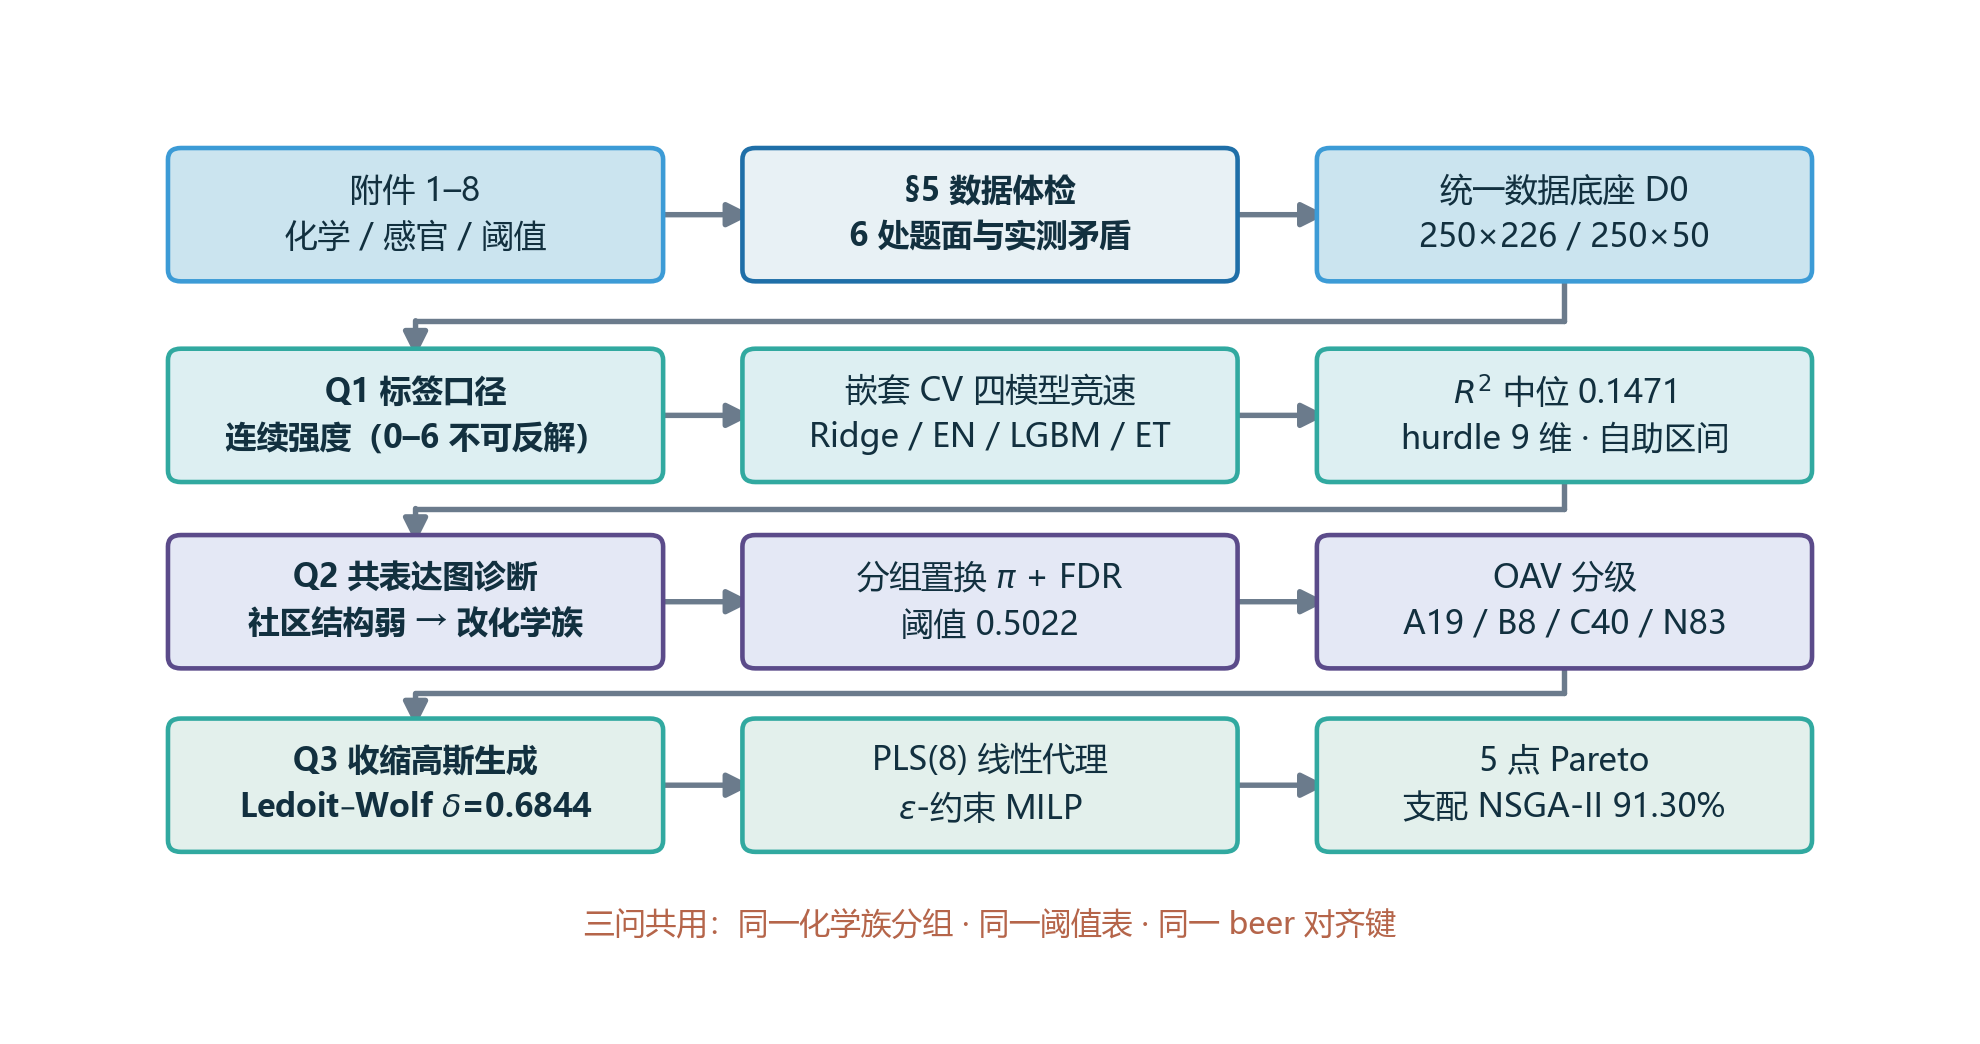
\includegraphics[width=\textwidth]{figures/fig_flow.png}
\caption{全文技术路线}
\label{fig:flow}
\end{figure}

\subsection{问题一的分析}

题目要求以附件1 的化合物数据为基础，给出附件3 中定义的 Aroma 与 Flavour 两套感官项的 0--6 分评分。这件事表面上是回归，实际有三层障碍。

第一层是标签不能直接用。附件4 给出的 50 个感官项并不是 0--6 的整数分，而是经过中心化的连续值：取值范围 $-2.151$ 到 $6.172$，六成是负数，每一列的不同取值少则 106 个、多则 250 个。本文试过把所有取值平移成非负数再四舍五入，结果中位 53.2\% 的样本被压到 0 分，分出来的等级几乎没有意义（第六章表~\ref{tab:q1grade} 有对照）；也试过先假定一个比例尺再取整，同样找不到稳定的比例尺。所以整数分不能从数据直接还原，只能另外定一套映射规则，并把这条限制写进论文。

第二层是样本少、特征多。250 款酒对 231 个化学指标，比值接近 1。这种规模下任何模型都能把训练集拟合得很好，所以评估方法比模型本身更关键，必须用嵌套交叉验证把选模型与报分数分开，组织方式见 6.3 节。

第三层是化学谱究竟能解释多少感官。同一数据集的原论文\cite{schreurs2024}报告梯度提升在训练感官面板上的多输出 $R^2$ 约 0.21 到 0.22，本文把它当作可比的参照水平：结果远低于它说明实现有问题，接近它则说明这是数据本身的信息量上限，换更复杂的模型也不会有实质改善。

据此确定了做法。候选模型取四个：岭回归与弹性网\cite{zou2005}代表线性方法，可解释性好但抓不住非线性；LightGBM 与 ExtraTrees 代表树集成，能抓非线性与交互，但在 250 个样本上容易过拟合。四个模型放进同一个嵌套交叉验证里横向比较，每个感官项各自取内层表现最好的那一个，而不是全篇强推一个模型。另外，有些感官项有大量样本压在最低值（例如 barnyard 有 47.6\% 的样本落在最小值附近），这类项用普通回归会把“没尝出来”和“尝到了但很弱”混在一起，本文对它们额外加一层“先判断有没有、再判断有多强”的两段式结构。

\subsection{问题二的分析}

题目要求用附件2 的相关矩阵建化合物网络，结合附件1 的特征，给出每个感官项最关键的三类化合物，并论证结果稳定、化学上讲得通。

先说一个容易走错的地方。附件8 里已经放了两张现成的化合物重要性排序 MDI 与 SHAP。直接取用最省力，但不适用：它们是全部 231 列对某一个综合目标的排序，不是对 50 个感官项分别排的，也不说明因果关系\cite{lundberg2017}；本文只留作最后的方向对照。

真正的难点是共线。231 个指标里有 219 个的方差膨胀因子大于 10，但只有 6 对相关系数的绝对值超过 0.9。这说明共线是一大片弱相关的累积，不是少数几列重复。因此逐列打乱不可用：被打乱的列会被同族其余列顶替，重要性系统性偏小\cite{strobl2008}。本文改为按附件8 的化学来源分组、同族一起打乱。

稳定性是题目点名要求的内容，本文用两种方式量化：一是自助重采样 200 次，每次重做“打乱—排序”，统计每个化合物进入前三名的次数比例；二是换模型后各排一次前十名，模型取 LightGBM、ExtraTrees 与岭回归，两两计算 Jaccard 系数。前者衡量换一批样本还稳不稳，后者衡量换一个模型还稳不稳。显著性阈值也不手工设定，而由稳定选择的有限样本界反解（见 7.3 节）\cite{meinshausen2010}。

最后要有化学上的说服力。本文用气味活性值\cite{grosch1994}判断，即浓度除以该物质的香气阈值，据以核查：统计上重要的化合物，是否真的浓到能被闻到，并与已报道的啤酒气味活性物清单\cite{kishimoto2018} 对照。这一步会否掉一部分结果，但否掉是应该的。

\subsection{问题三的分析}

题目要求以风格为条件学一个生成模型，在给定风格下生成合理的化合物谱并给出感官画像，再做跨风格迁移且保证缺陷物不恶化。

生成这一步的困难在样本量。22 个风格里最小的只有 3 款酒，即 Faro 风格，多数不超过 20 款。条件变分自编码器、条件生成对抗网络这类方法用在这种规模上无法估计条件分布\cite{xu2019}，本文把它们作为对照并在论文中明确写“不适用”，不作为主方法。实际采用的做法更朴素：在每个风格内部估计一个多元正态分布，协方差用 Ledoit--Wolf 收缩法\cite{ledoit2004}估计。收缩的意义是，样本少的时候直接用样本协方差会严重高估方差方向，收缩后向对角阵靠拢，生成样本不会离实测太远；收缩强度由数据算出，不手工设定。

生成之后要判断像不像。本文用最近邻距离检验：如果生成的样本与最近的实测样本距离远小于实测彼此之间的距离，说明它在复制；远大于则说明跑到了数据分布之外。两者都不可接受，理想情况是两者相当。

优化这一步要有感官目标。本文用偏最小二乘回归\cite{wold2001}建立一个从化学谱到 50 项感官的线性映射，取 8 个成分，系数可以直接写进优化模型的约束。之所以选偏最小二乘而不选树模型，是因为后面要解的是线性混合整数规划，需要可线性化的结构，树模型无法写进规划。

三个目标分别是感官偏差、缺陷风险和改动代价，单位不同、不能相加，因此用 $\varepsilon$-约束法\cite{mavrotas2009}：先分别求三个单目标得到支付表，再在对缺陷风险和改动代价的限制下逐步收紧，逐点求最小的感官偏差。这里之所以不直接用 Gurobi 自带的多目标接口，是因为它只支持线性目标，而感官偏差含绝对值，需要先线性化并入约束。为了验证这套精确解是否值得，本文另外手写了一个 NSGA-II\cite{deb2002}作对照，用两套前沿的支配关系与超体积来判断。
